\begin{frame}{2º Ciclo}
	\begin{columns}
		\column{.5\textwidth}
        Ciclo Otimizado
		\column{.5\textwidth}
		\begin{figure}[hb]
      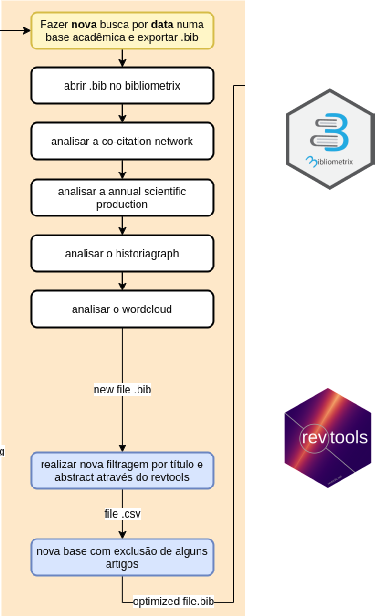
\includegraphics[width=0.65\textwidth]{figures/ciclo2.png}
		\end{figure}
	\end{columns}
\end{frame}

\begin{frame}{2º Ciclo - Nova Busca}
  \begin{figure}[hb]
    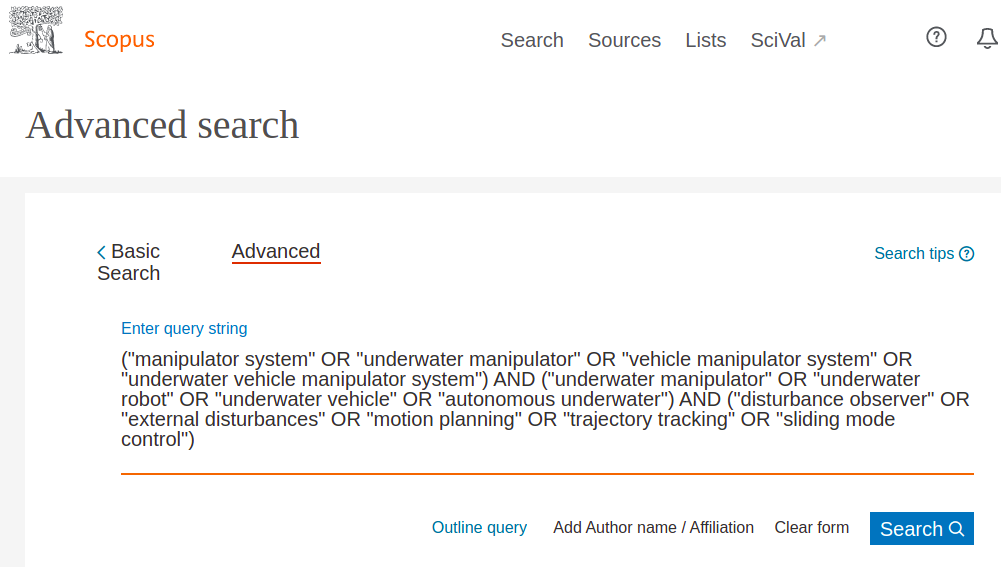
\includegraphics[width=1\textwidth]{figures/novabusca.png}
  \end{figure}

\end{frame}

\begin{frame}{2º Ciclo - Bibliometrix}
	Importar o novo .bib
  \begin{figure}[hb]
			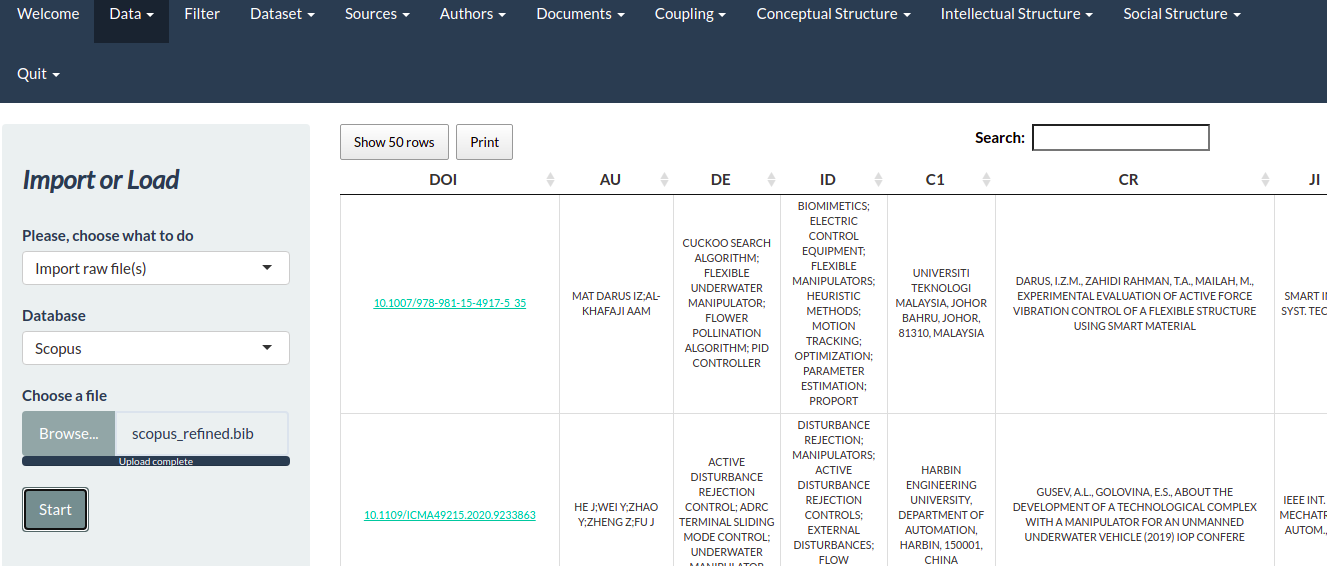
\includegraphics[width=1\textwidth]{figures/bibliometrix/b4.png}
  \end{figure}
\end{frame}

\begin{frame}{2º Ciclo - Bibliometrix}
	Analisar o Co-Citation Network
	\begin{columns}
		\column{.5\textwidth}
		\begin{figure}[hb]
      1º Ciclo
			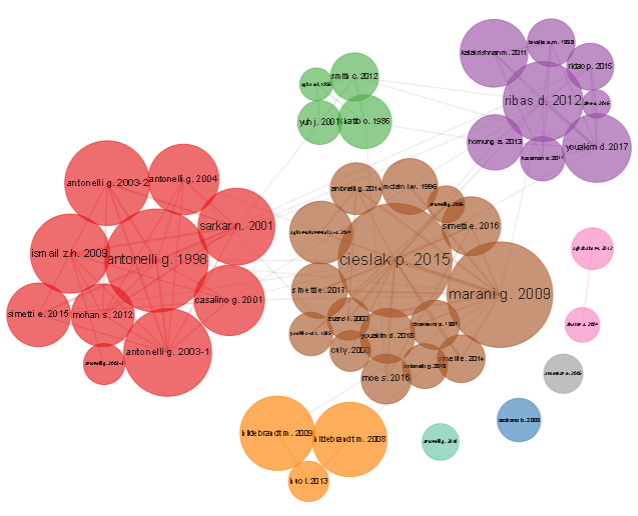
\includegraphics[width=1\textwidth]{figures/bibliometrix/brede1.png}
		\end{figure}
		\column{.5\textwidth}
		\begin{figure}[ht]
      2º Ciclo
			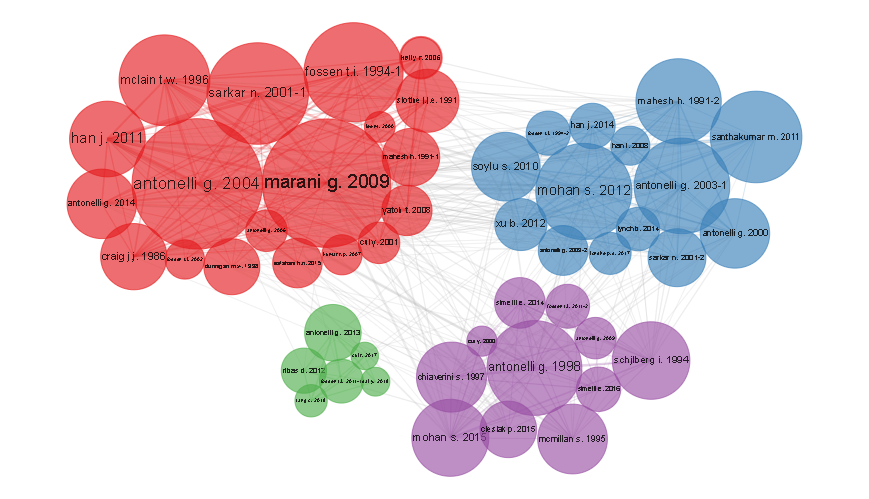
\includegraphics[width=1\textwidth]{figures/bibliometrix/brede2.png}
		\end{figure}
	\end{columns}
\end{frame}

\begin{frame}{2º Ciclo - Bibliometrix}
	Analisar o novo Annual Scientific Production
	\begin{columns}
		\centering
		\column{.5\textwidth}
		\begin{figure}[hb]
      		1º Ciclo
			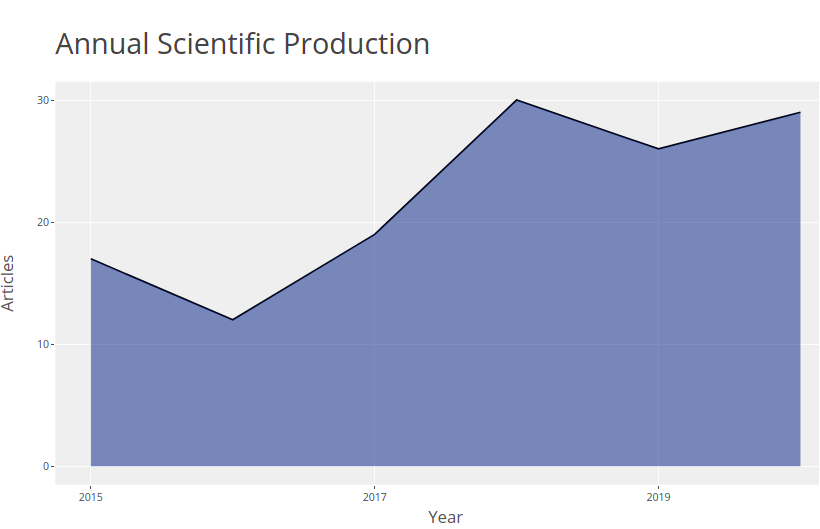
\includegraphics[width=1\textwidth]{figures/anualold.png}
		\end{figure}
		\column{.5\textwidth}
		\begin{figure}[ht]
      	2º Ciclo
      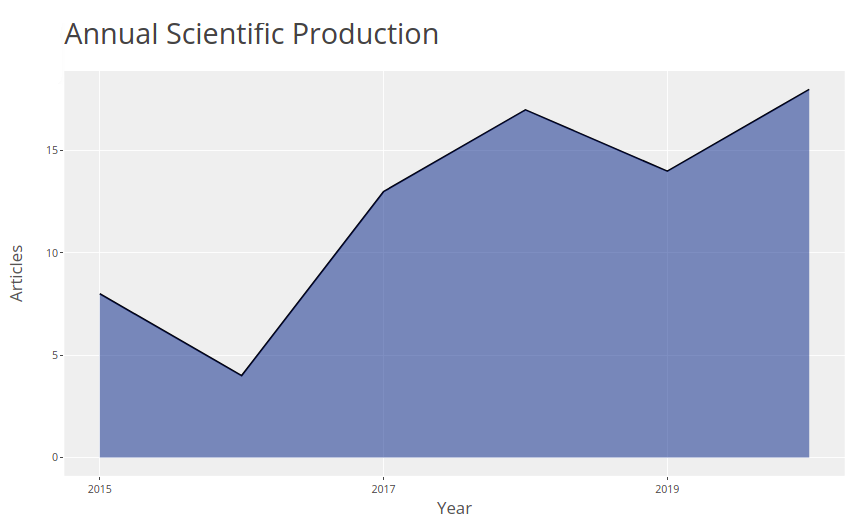
\includegraphics[width=1\textwidth]{figures/anualnovo.png}
		\end{figure}
	\end{columns}
\end{frame}

\begin{frame}{2º Ciclo - Bibliometrix}
	Analisar o Historiagraph
	\begin{columns}
		\column{.5\textwidth}
		\begin{figure}[hb]
      1º Ciclo
			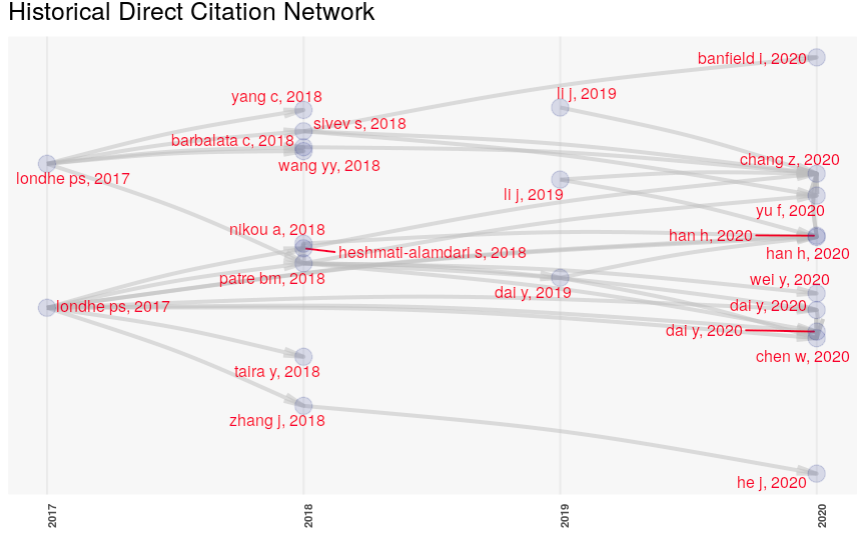
\includegraphics[width=1\textwidth]{figures/histold.png}
		\end{figure}
		\column{.5\textwidth}
		\begin{figure}[ht]
      2º Ciclo
      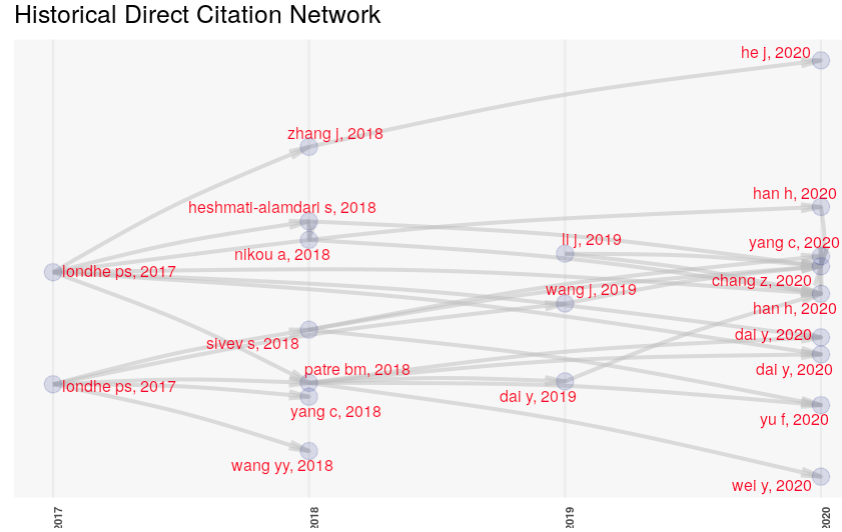
\includegraphics[width=1\textwidth]{figures/histnovo.png}
		\end{figure}
	\end{columns}
\end{frame}

\begin{frame}{2º Ciclo - Bibliometrix}
	Analisar o WorldCloud
	\begin{columns}
		\column{.5\textwidth}
		\begin{figure}[hb]
      1º Ciclo
			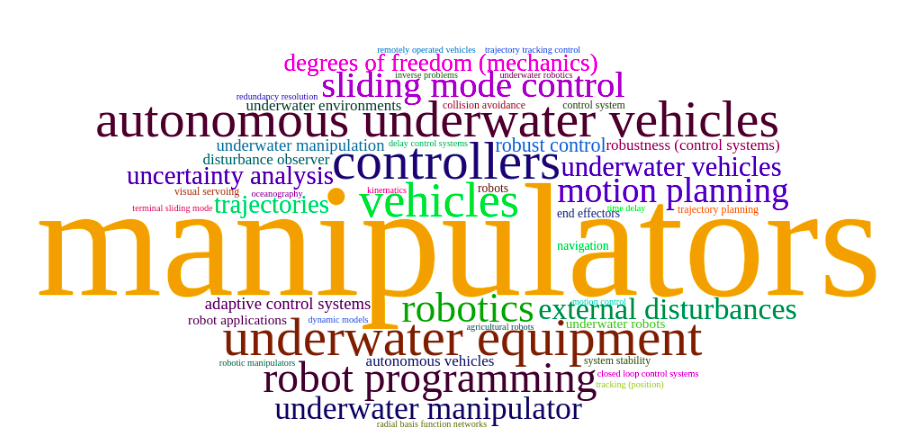
\includegraphics[width=1\textwidth]{figures/worldold.png}
		\end{figure}
		\column{.5\textwidth}
		\begin{figure}[ht]
      2º Ciclo
      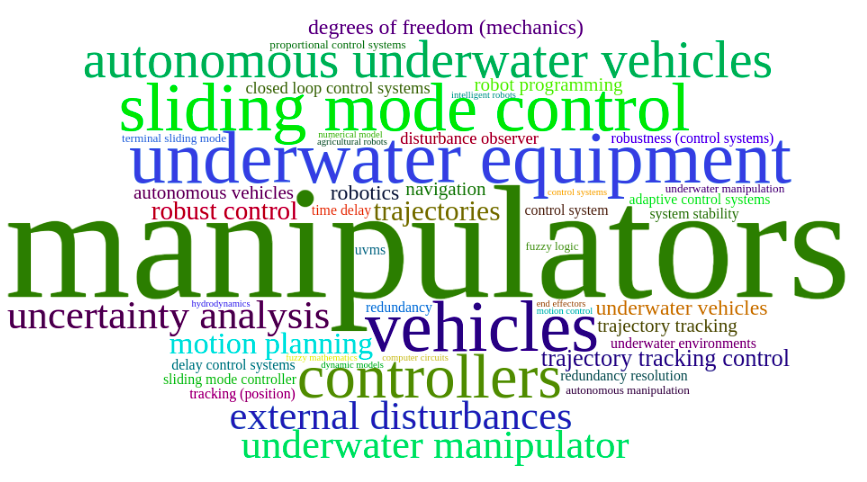
\includegraphics[width=0.9\textwidth]{figures/worldnovo.png}
		\end{figure}
	\end{columns}
\end{frame}

\begin{frame}{2º Ciclo}
	\begin{columns}
		\column{.5\textwidth}
        Ciclo Otimizado
		\column{.5\textwidth}
		\begin{figure}[hb]
      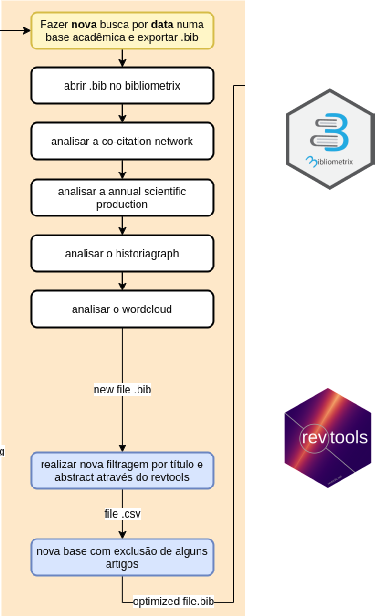
\includegraphics[width=0.65\textwidth]{figures/ciclo2.png}
		\end{figure}
	\end{columns}
\end{frame}

\begin{frame}{2º Ciclo - RevTools}
  \begin{columns}
		\column{.5\textwidth}
    \begin{itemize}
      \item É um pacote de R para apoiar pesquisadores que trabalham em projetos de síntese de evidências
      \item Visualizar padrões em dados bibliográficos
      \item Selecionar ou excluir interativamente artigos ou palavras individuais 
    \end{itemize}
    
    \column{.5\textwidth}
    \begin{figure}[hb]
      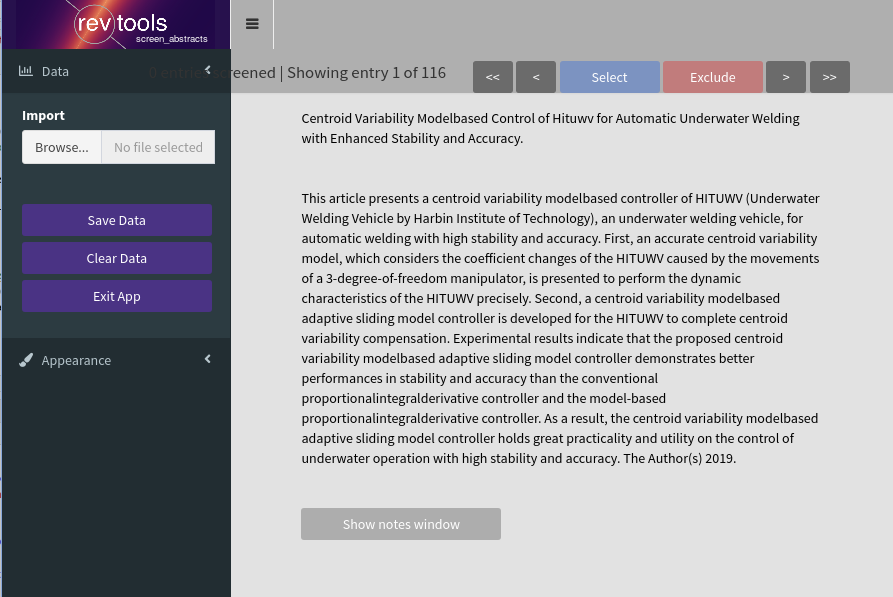
\includegraphics[width=1\textwidth]{figures/revtools.png}
		\end{figure}
	\end{columns}

\end{frame}

\begin{frame}{2º Ciclo - RevTools}
  Realizar uma nova filtragem por título e resumo através do RevTools. \\
  Nova base com exclusão de alguns artigos.
  \begin{figure}[hb]
    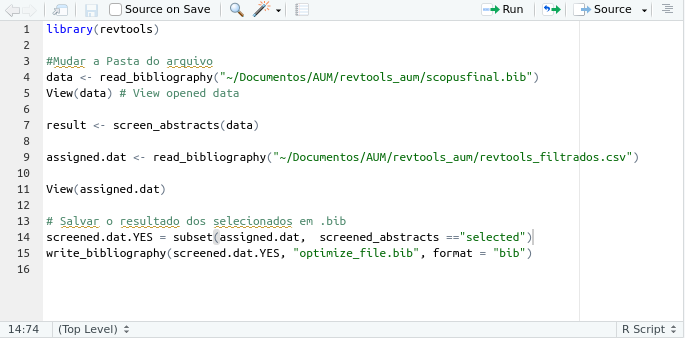
\includegraphics[width=1\textwidth]{figures/revtoolscod.png}
  \end{figure}

\end{frame}
